\documentclass{yResume}
%===============================================================================
% choose language photo
% options: XXXtrue
% use \lang{english}{中文} to select language
% if not specific, this paragraph will be used in two language
%===============================================================================
% \englishtrue{}
\phototrue{}
%===============================================================================
% title and footer lauguage
%===============================================================================
\name{\lang{Jack Ha}{姓名}}
% \ifenglish{}
%   \CTEXoptions[today=old]  
%   % TODO
% 	\name{Jack Ma}
% \else 
%   % TODO
%   \name{姓名}
% \fi
%===============================================================================
% 正文部分
%===============================================================================
\begin{document}
\begin{resume}
%===============================================================================
% 个人信息
% 可选项:\twocontact\threecontact\fourcontact\eightcontact\ninecontact
% \sixxcontact(3行)\sixcontact(2行)
% 内容: \address\phone\email\person(age,sex,native,etc)
% \homepage\facebook\github\linkedin\twitter\wechat\weibo\qq
% 照片: 如果 \phototrue{} 将图片放入根目录 并改名(默认为1.jpg)
%===============================================================================
{
  \large
  \it
  \ifphoto{}
    \begin{minipage}{0.84\textwidth}
      \myname{}
      \sixxcontact{\lang{\address{city,street,location}}{\address{城市,街道,地点}}}
        {\phone{+86 138{-}8888{-}8888}}
        {\wechat{wechat account}}
        {\email{example@example.com}}
        {\twitter{twitter account}}
        {\github{git account}}
    \end{minipage}
    \begin{minipage}{0.14\textwidth}
      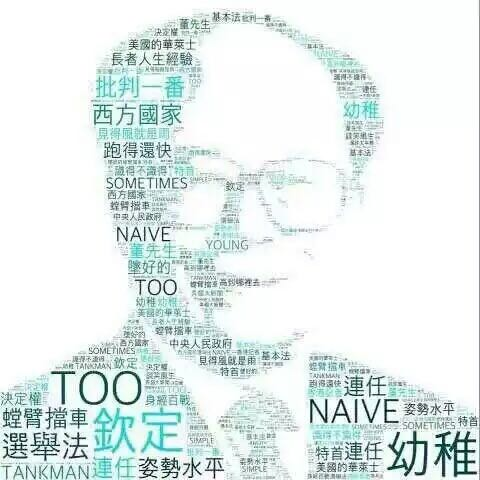
\includegraphics[width=\textwidth]{1.jpg}
    \end{minipage}
  \else
    \myname{}   
    \sixcontact{\lang{\address{city,street,location}}{\address{城市,街道,地点}}}
      {\phone{+86 138{-}8888{-}8888}}
      {\wechat{wechat account}}
      {\email{example@example.com}}
      {\twitter{twitter account}}
      {\github{git account}}
  \fi
  \par
}
%===============================================================================
% 全文本内容(可自由按照需求组合)

% \ytitle :带横线的大标题
% \yparagraph :正文段落
% \ysubtitle :小标题
% \ytimeline :生成2行(格式为:项目/细节           时间/地点)
% \yitem :使用列表列出
%===============================================================================

%===============================================================================
% 推荐排版模式
%===============================================================================

% plan 1
\ytitle{\lang{title}{题目}}
\lang{
  \yparagraph{We describe a quantum key distribution protocol based on pairs of entangled qubits that generates a secure key between two partners in an environment of unknown and slowly varying reference frame. A direction of particle delivery is required, but the phases between the computational basis states need not be known or fixed. The protocol can simplify the operation of existing setups and has immediate applications to emerging scenarios such as earth-to-satellite links and the use of integrated photonic waveguides.}
  \ysubtitle{sub title}
  \yparagraph{A direction of particle delivery is required, but the phases between the computational basis states need not be known or fixed. }
}{
  \yparagraph{我们描述了一种基于纠缠量子比特对的量子密钥分发协议,该协议在未知和缓慢变化的参考帧的环境中在两个伙伴之间生成安全密钥。需要粒子传递的方向,但是不需要知道或修复计算基础状态之间的相位。该协议可以简化现有设置的操作,并立即应用于新兴的场景,如地对卫链路和集成光子波导的使用。}
  \ysubtitle{副标题}
  \yparagraph{需要粒子传递的方向,但是不需要知道或修复计算基础状态之间的相位。该协议可以简化现有设置的操作,并立即应用于新兴的场景,如地对卫链路和集成光子波导的使用。}
}

% plan 2
\ytitle{\lang{title}{题目}}
\ytimeline{\lang{Project}{项目}}{\lang{Specific}{细节}}{2017.6--2017.9}{\lang{Place}{地点}}
\lang{
  \yparagraph{We describe a quantum key distribution protocol based on pairs of entangled qubits that generates a secure key between two partners in an environment of unknown and slowly varying reference frame. A direction of particle delivery is required, but the phases between the computational basis states need not be known or fixed. The protocol can simplify the operation of existing setups and has immediate applications to emerging scenarios such as earth-to-satellite links and the use of integrated photonic waveguides.}
}{
  \yparagraph{我们描述了一种基于纠缠量子比特对的量子密钥分发协议,该协议在未知和缓慢变化的参考帧的环境中在两个伙伴之间生成安全密钥。需要粒子传递的方向,但是不需要知道或修复计算基础状态之间的相位。该协议可以简化现有设置的操作,并立即应用于新兴的场景,如地对卫链路和集成光子波导的使用。}
}
\ytimeline{\lang{Project}{项目}}{\lang{Specific}{细节}}{2017.6--2017.9}{\lang{Place}{地点}}
\ylist{
  \lang{
    \item We describe a quantum key distribution protocol based on pairs of entangled qubits
    \item We describe a quantum key distribution protocol based on pairs of entangled qubits
    \item We describe a quantum key distribution protocol based on pairs of entangled qubits
    \item We describe a quantum key distribution protocol based on pairs of entangled qubits
  }{
    \item 我们描述了一种基于纠缠量子比特对的量子密钥分发协议
    \item 我们描述了一种基于纠缠量子比特对的量子密钥分发协议
    \item 我们描述了一种基于纠缠量子比特对的量子密钥分发协议
    \item 我们描述了一种基于纠缠量子比特对的量子密钥分发协议
  }  
}
% plan 3
\ytitle{\lang{title}{题目}}
\lang{
  \yevent{CFA}{contant,what happend here}{1999}
  \ylist{\item We describe a quantum key distribution protocol}
  \yevent{CFA}{contant,what happend here}{1999}
  \yparagraph{We describe a quantum key distribution protocol based on pairs of entangled qubits that generates a secure key between two partners in an environment of unknown and slowly varying reference frame. A direction of particle delivery is required, but the phases between the computational basis states need not be known or fixed. The protocol can simplify the operation of existing setups and has immediate applications to emerging scenarios such as earth-to-satellite links and the use of integrated photonic waveguides.}
  \yevent{CFA}{contant,what happend here}{1999}
  \yevent{CFA}{contant,what happend here}{1999}
}{
  \yevent{测试}{具体内容}{1999}
  \ylist{\item 具体内容是什么}
  \yevent{测试}{具体内容}{1999}
  \yevent{测试}{具体内容}{1999}
  \yparagraph{我们描述了一种基于纠缠量子比特对的量子密钥分发协议,该协议在未知和缓慢变化的参考帧的环境中在两个伙伴之间生成安全密钥。需要粒子传递的方向,但是不需要知道或修复计算基础状态之间的相位。该协议可以简化现有设置的操作,并立即应用于新兴的场景,如地对卫链路和集成光子波导的使用。}
  \yevent{测试}{具体内容}{1999}
}
% plan 4
\ytitle{\lang{title}{题目}}
\ytimeline{\lang{title of Paper}{论文的题目}}{\lang{Details of the paper}{文章细节}}{2018.11}{Physics Review Letter}
\ytimeline{\lang{title of Paper}{论文的题目}}{\lang{Details of the paper}{文章细节}}{2018.11}{Physics Review Letter}
\ytimeline{\lang{title of Paper}{论文的题目}}{\lang{Details of the paper}{文章细节}}{2018.11}{Physics Review Letter}
\ytimeline{\lang{title of Paper}{论文的题目}}{\lang{Details of the paper}{文章细节}}{2018.11}{Physics Review Letter}
\end{resume}
\end{document}